%! alt Two circles with the same centre O, drawn with inner radius 12. The lower horizontal line crosses the outer circle at A and D and the inner circle at B and C, with AB = 3 and BC = 21; the perpendicular from O meets it at M, the midpoint of both chords. A second, slanting line crosses the outer circle at P and S and the inner circle at Q and R; the perpendicular from O meets it at N, and the inner circle cuts PS into three equal parts PQ = QR = RS = 6, so PS = 18. For both lines the squared distance from the foot to an outer point minus the squared distance to an inner point is 72.
%! after_paragraph 1
%! scale 1/4
%! let h = sqrt(135)
% The shared preamble of every Cevian figure. pipeline/figures turns these colours into theme-aware paint,
% and refuses any other colour, so draw only with them:
%   figink (lines and labels), figaux (construction lines), figaccent (the object the argument turns on),
%   figtint and figaccenttint (light fills).
\documentclass[border=1.5pt]{standalone}
\usepackage{tkz-euclide}
\definecolor{figink}{RGB}{0,0,0}
\definecolor{figaux}{RGB}{85,85,85}
\definecolor{figaccent}{RGB}{192,57,43}
\definecolor{figtint}{RGB}{221,221,221}
\definecolor{figaccenttint}{RGB}{245,213,208}
% tkz-euclide's defaults draw circles, compasses and marks in 50% grey and fill points with a tint.
\makeatletter
\def\tkz@otherlinecolor{figink}
\def\tkz@euc@circlecolor{figink}
\def\tkz@euc@compasscolor{figink}
\def\tkz@euc@mkcolor{figink}
\def\tkz@mk@fill{figink}
\def\tkz@euc@pointfillcolor{figink}
\makeatother
\tkzSetUpLine[color=figink,line width=.7pt]
\tkzSetUpArc[color=figink,line width=.7pt]
\tkzSetUpCompass[color=figink,line width=.5pt]
\tkzSetUpPoint[color=figink,fill=figink,size=3.1pt]
\tikzset{
  every picture/.style={line cap=round,line join=round,color=figink},
  circle style/.append style={color=figink,line width=.7pt},
  aux/.style={color=figaux,line width=.45pt,dash pattern=on 2.6pt off 2pt},
  key/.style={color=figaccent,line width=1pt},
  mk/.style={color=figink,line width=.5pt},
  lbl/.style={color=figink,inner sep=2.2pt},
  len/.style={color=figink,inner sep=1.5pt,font=\small},
}

\begin{document}
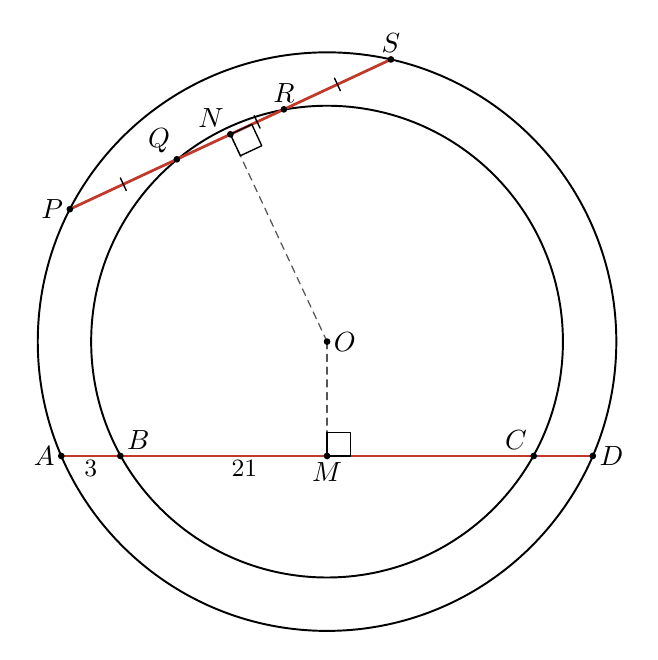
\begin{tikzpicture}
\tkzDefPoint(0.0,0.0){O} %! O = (0, 0)
\tkzDefPoint(0.0,-1.4523688){M} %! M = (0, -h/2)
\tkzDefPoint(-3.3750000,-1.4523688){A} %! A = (-27/2, -h/2)
\tkzDefPoint(-2.6250000,-1.4523688){B} %! B = (-21/2, -h/2)
\tkzDefPoint(2.6250000,-1.4523688){C} %! C = (21/2, -h/2)
\tkzDefPoint(3.3750000,-1.4523688){D} %! D = (27/2, -h/2)
\tkzDefPoint(-1.2275951,2.6325862){N} %! N = rotate((0, h), O, 25)
\tkzDefPoint(-3.2667876,1.6816951){P} %! P = rotate((-9, h), O, 25)
\tkzDefPoint(-1.9073260,2.3156225){Q} %! Q = rotate((-3, h), O, 25)
\tkzDefPoint(-0.54786428,2.9495499){R} %! R = rotate((3, h), O, 25)
\tkzDefPoint(0.81159740,3.5834773){S} %! S = rotate((9, h), O, 25)
%! fact on_circle(A, O, sqrt(216))
%! fact on_circle(D, O, sqrt(216))
%! fact on_circle(P, O, sqrt(216))
%! fact on_circle(S, O, sqrt(216))
%! fact on_circle(B, O, 12)
%! fact on_circle(C, O, 12)
%! fact on_circle(Q, O, 12)
%! fact on_circle(R, O, 12)
%! fact collinear(B, A, D)
%! fact collinear(C, A, D)
%! fact collinear(Q, P, S)
%! fact collinear(R, P, S)
%! fact dist(A, B) == 3
%! fact dist(B, C) == 21
%! fact dist(P, Q) == 6
%! fact dist(Q, R) == 6
%! fact dist(R, S) == 6
%! fact dist(P, S) == 18
%! fact perp(O, M, A, D)
%! fact perp(O, N, P, S)
%! fact midpoint(M, A, D)
%! fact midpoint(M, B, C)
%! fact midpoint(N, P, S)
%! fact midpoint(N, Q, R)
%! fact dist(O, A)**2 - dist(O, B)**2 == 72
%! fact dist(M, A)**2 - dist(M, B)**2 == 72
%! fact dist(N, P)**2 - dist(N, Q)**2 == 72
\tkzDrawCircle(O,A)
\tkzDrawCircle(O,B)
\tkzDrawSegment[aux](O,M)
\tkzDrawSegment[aux](O,N)
\tkzDrawSegment[key](A,D)
\tkzDrawSegment[key](P,S)
\tkzMarkRightAngle[size=.3,mk](O,M,D)
\tkzMarkRightAngle[size=.3,mk](O,N,S)
\tkzMarkSegments[mark=|,size=2.5pt,mk](P,Q R,S)
\tkzMarkSegment[mark=|,size=2.5pt,pos=.75,mk](Q,R)
\tkzDrawPoints(O,M,N,A,B,C,D,P,Q,R,S)
\tkzLabelPoint[right,lbl](O){$O$}
\tkzLabelPoint[below,lbl](M){$M$}
\tkzLabelPoint[above left,lbl](N){$N$}
\tkzLabelPoint[left,lbl](A){$A$}
\tkzLabelPoint[above right,lbl](B){$B$}
\tkzLabelPoint[above left,lbl](C){$C$}
\tkzLabelPoint[right,lbl](D){$D$}
\tkzLabelPoint[left,lbl](P){$P$}
\tkzLabelPoint[above left,lbl](Q){$Q$}
\tkzLabelPoint[above,lbl](R){$R$}
\tkzLabelPoint[above,lbl](S){$S$}
\tkzLabelSegment[below,len](A,B){$3$}
\tkzLabelSegment[below,pos=.3,len](B,C){$21$}
\end{tikzpicture}
\end{document}
